\chapter{Interaction gaussienne avec champ magnétique confinant}
\label{sec_laser}

Jusqu'à présent nous avons développé le modèle Solid-On-Solid et étudié ses propriétés pour des modèles d'interface en présence d'un champ magnétique uniforme, le potentiel chimique. Dans ce chapitre, nous étudions les propriétés d'un champ magnétique non-uniforme en analogie à certaines expériences effectuées au Laboratoire Onde Matière d'Aquitaine par l'équipe de Jean-Pierre Delville. Dans ces expériences, un liquide quaternaire composé de toluenne, sodium dodecyl sulfate, n-butanol et eau possède proche du point critique deux phases miscellaires séparées avec une tension de surface de $\sigma \simeq 10^{-7}N/m$ pour $T-T_C=1.5K$\cite{casner_laser-induced_2003,delville_laser_2009,girot_conical_2019}. À cela s'ajoute un laser qui par pression de radiation pousse une phase dans l'autre. 

Dans un système de taille $L'\times L$, avec $y \in [-\frac{L}{2},\frac{L}{2}]$ \footnotetext{Lorsqu'il s'agit de diagonaliser la matrice de transfert, il suffit de faire la translation $y \to y+\frac{L}{2}$}. Nous nous proposons d'étudier les propriétés statistiques d'une telle interface grâce à la présence d'un champ magnétique de la forme 
\begin{align}
	V(\sigma_{x,y}) = B \sgn(y)
\end{align}
qui se traduit dans le formalisme SOS par
\begin{align}
    V(h_i) = B |h_i|
    \label{staged}
\end{align}
similaire à l'équaiton \ref{neggstaged}, où cette fois le champ magnétique confine l'interface au voisinage de $0$.

Dans ce chapitre, nous étudions analytiquement la distribution de l'interface, le spectre d'énergie et la fonction de corrélation de ce système, qui nous permet de trouver une dépendance entre la tension superficielle avec la température et l'intensité $B$ du champ magnétique. Puisque le système expérimental possède un régime hors-équilibre, nous étudions également l'effet d'un écoulement uniforme au niveau de l'interface. 

%%%%%%%%%%%%%%%%%%%%%%%%%%%%%%%%
    \section{Interface statique}
    \subsection{Distribution de probabilité de l'interface}
%%%%%%%%%%%%%%%%%%%%%%%%%%%%%%%%


Grâce au potentiel \ref{staged}, l'interface est localisée autour de $h=0$, et possède une distribution symmétrique. La méthode décrite à la section \ref{par-stab} pour trouver la forme de la distribution nécessite au préalable un ansatz de la solution. Nous proposons ici une méthode plus puissante qui repose sur des équations continues. Dans le cas où la largeur de l'interface est grande par rapport à l'unité, on s'attend à ce que la description possède les mêmes propriétés que le système discontinu qu'est le modèle Solid-On-Solid.

Une manière de se représenter une configuration de l'interface est de le comparer à la trajectoire d'un marcheur brownien commençant au point $h_0$ et se déplaçant sur $L'$ pas de temps discontinus, jusqu'à arriver à sa position finale $h_L$, avec une trajectoire périodique de période $L'$. La fonction de partition se comprend maintenant comme la somme des trajectoires du marcheur brownien au lieu de la somme des configurations de l'interface. On associe à la trajectoire l'énergie $E = \sigma \mathcal{L}$, où $\sigma$ est la tension superficielle de notre interface et $\mathcal{L}$ la distance totale parcourue par la particule browniene. D'un point de vue continu, la distance effectuée pour de petits déplacements est $d\mathcal{L} = \sqrt{1+\frac{dh^2}{dx^2}} dx \simeq h'^2 dx$.
L'Hamiltonien discret correspondant devient gaussien
\begin{align}
    H = J \sum_i (h_i-h_{i+1})^2 + B \sum_i \frac{|h_i|+|h_{i+1}|}{2}
    \label{hamil-gauss}
\end{align}
tandis qu'une version continue du problème est 
\begin{align}
	H = \frac{\sigma}{2} \int_0^{L'} h'^2(x) dx + B \int_0^{L'} |h(x)|dx
\end{align}

{\color{red} Dans tout ce qui suit, peut-on juste mettre $\sigma \to 2 \sigma$ et enlever le facteur 2 de partout dans les équations ? Ça allège toutees les notations.}

La fonction de partition de toutes les trajectoires $h(x)$ possibles de notre particule telles que $h(0)=h(L')=h^\ast$ est alors donné par
\begin{align}
	\mZ(h,h^\ast,L') = \int_{h(0)=h} d[h] \delta(h(L')-h^\ast)e^{-\frac{\beta \sigma}{2} \int_0^{L'} h'^2(x) dx -\beta B \int_0^{L'} |h(x)|dx}
\end{align}
avec la condition initiale $\mZ(h,h',0)=\delta(h-h')$. La fonction de partition $\mZ$ obéit alors à l'équation de Schrödinger temporelle
\begin{align}
	\frac{\partial \mZ}{\partial {L'}} = \frac{1}{2 \beta \sigma} \frac{\partial^2 \mZ}{\partial h^2}  - B \beta |h| \mZ
\end{align}
avec la condition initiale $\mZ(h,h',0) = \delta(h-h')$.  En absence d'un potentiel externe on retrouve les solutions en sinus et cosinus décrivant une interface délocalisée à travers tout le système, comme dans l'équation \ref{lambda-sos}. En décomposant la fonction de partition dans la base des solutions stationnaires $\psi_E$ correspondant aux énergies propres $E$ 
\begin{align}
	Z(h,h',L') = \sum_E e^{-EL'}\psi_E(h) \psi_E(h')
	\label{schro_temp}
\end{align}
on obtient l'équation aux états propres
\begin{align}
	\epsilon \psi_\epsilon = - \frac{1}{2} \frac{\partial^2 \psi_\epsilon}{\partial h^2} + \lambda |h| \psi_\epsilon
\end{align}
où l'équation a été admiensionalisée par $\epsilon = E\beta\sigma$ et $\lambda=\beta^2 \sigma B$. À nouveau, dans la limite thermodynamique, seul l'état fondamental $E_0$ contribue à la distribution des hauteurs $p(h) = \psi_{E_0}^2(h)$.
Les solutions sont données par les fonctions d'ondes symmétriques par rapport à $h=0$
\begin{align}
	\psi_\epsilon (h) = Ai \left( (2\lambda)^\frac{1}{3}(|h|-\frac{\epsilon}{\lambda}) \right)
\end{align}
où $Ai(x)$ est la fonction de Airy. 

\begin{figure}[t]
	\begin{minipage}[t]{0.5\linewidth}
        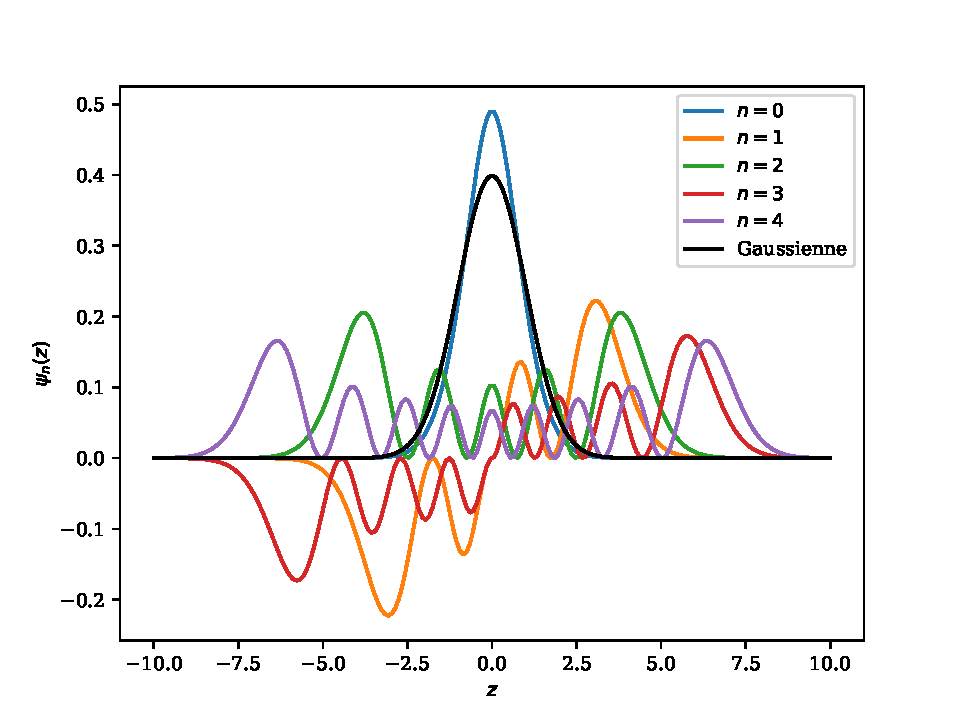
\includegraphics[width=\linewidth]{sosequi-laser/etats-laser.pdf}
	\end{minipage}%
	\begin{minipage}[t]{0.5\linewidth}
    	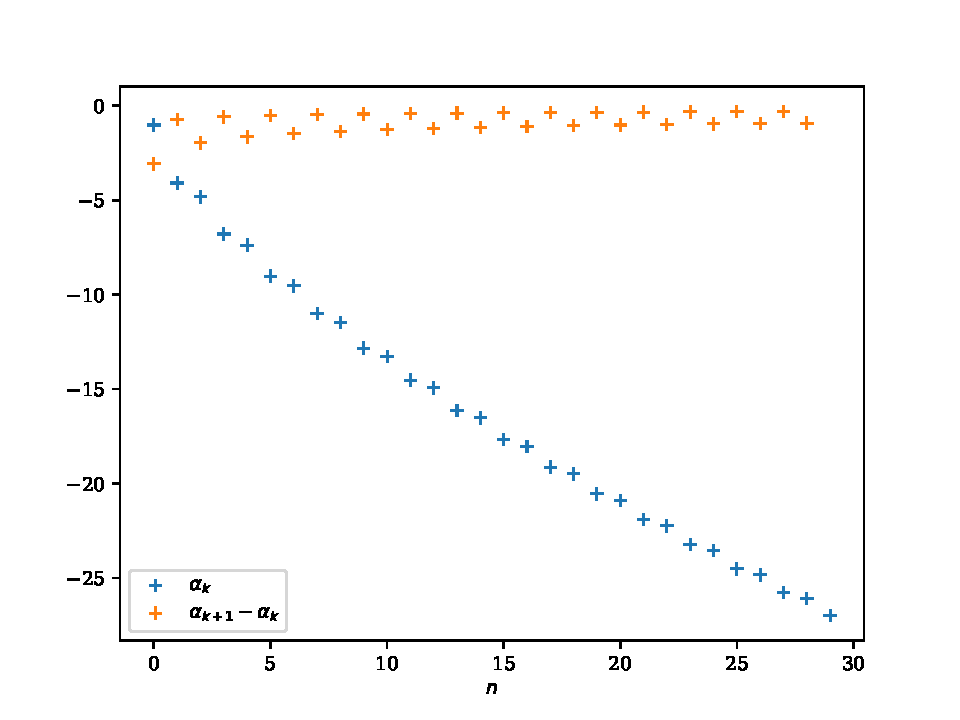
\includegraphics[width=\linewidth]{sosequi-laser/energies-laser.pdf}
	\end{minipage}
    \caption{À gauche, états propres $\psi_n$ avec en noir, une référence par rapport à la distribution gaussienne. À droite, la série $\alpha_n$.}
	\label{fig-airy}    
\end{figure}

Par analogie avec l'oscillateur harmonique quantique, nous cherchons des solutions avec des conditions aux limites $\psi'_\epsilon(0) = 0$ pour les états pairs et $\psi_\epsilon(0) = 0$ pour les états impairs. Cela nous donne $\epsilon_n = 2^{-\frac{1}{3}} \lambda^\frac{2}{3}\alpha_n$ où $-\alpha_{2n} \greater 0$ est le 2n-ième zéro de la dérivée de la fonction d'Airy Ai' et $-\alpha_{2n+1} \greater 0$ est le (2n+1)-ième zéro de la fonction d'Airy Ai (voir figure \ref{fig-airy}). L'état fondamental est donné par le plus petit zéro de la fonction $\alpha_0 \simeq 1.0187$ et a une énergie de 
\begin{align}
	E_0 = \frac{\epsilon_0}{\beta \sigma} = 2^{-\frac{1}{3}} \alpha_0 \beta^\frac{1}{3}\sigma^{\frac{1}{3}}B^\frac{2}{3}
\end{align}
L'état fondamental s'écrit alors
\begin{align}
	\psi_0(h) = \frac{ Ai ( (2\lambda)^\frac{1}{3} |h|-\alpha_0 )}{ \sqrt{2 \int_0^\infty dh Ai^2 ( (2\lambda)^\frac{1}{3} |h|-\alpha_0 ) }}
\end{align}
où le dénominateur est une constante de normalisation utilisant la symétrie $p(h)=p(-h)$.  
On peut calculer les états excités suivants suivant leur parité, les états pairs s'écrivant
\begin{align}
	\psi_{2n}(h) = \frac{ Ai ( (2\lambda)^\frac{1}{3} |h|-\alpha_{2n} )}{ \sqrt{2 \int_0^\infty dh Ai^2 ( (2\lambda)^\frac{1}{3} h-\alpha_{2n} ) }}
\end{align}
et les états impairs
\begin{align}
	\psi_{2n+1}(h) = \frac{ \sgn(h) Ai ( (2\lambda)^\frac{1}{3} |h|-\alpha_{2n+1} )}{ \sqrt{2 \int_0^\infty dh Ai^2 ( (2\lambda)^\frac{1}{3} h-\alpha_{2n+1} ) }}
\end{align}
d'énergie $E_{n} = E_0 \frac{\alpha_{n}}{\alpha_0}$. 

On peut adimensionner la distribution des hauteurs par $z = (2\lambda)^\frac{1}{3}h$, et on peut définir une largeur caractéristique de l'interface 
\begin{align}
	\xi_\perp = \frac{1}{(2\beta^2 \sigma B)^\frac{1}{3}}
	\label{xi_perp}
\end{align}


Dans la limite thermodynamique, la distribution des hauteurs  devient 
\begin{align}
	p(z) = \psi_0^2(z) = \frac{ Ai^2 ( |z|-\alpha_0 )}{ 2 \int_0^\infty dz Ai^2 ( z-\alpha_0 ) }
	\label{airy}
\end{align}
	
\begin{figure}[t]
	\begin{minipage}[t]{0.5\linewidth}
		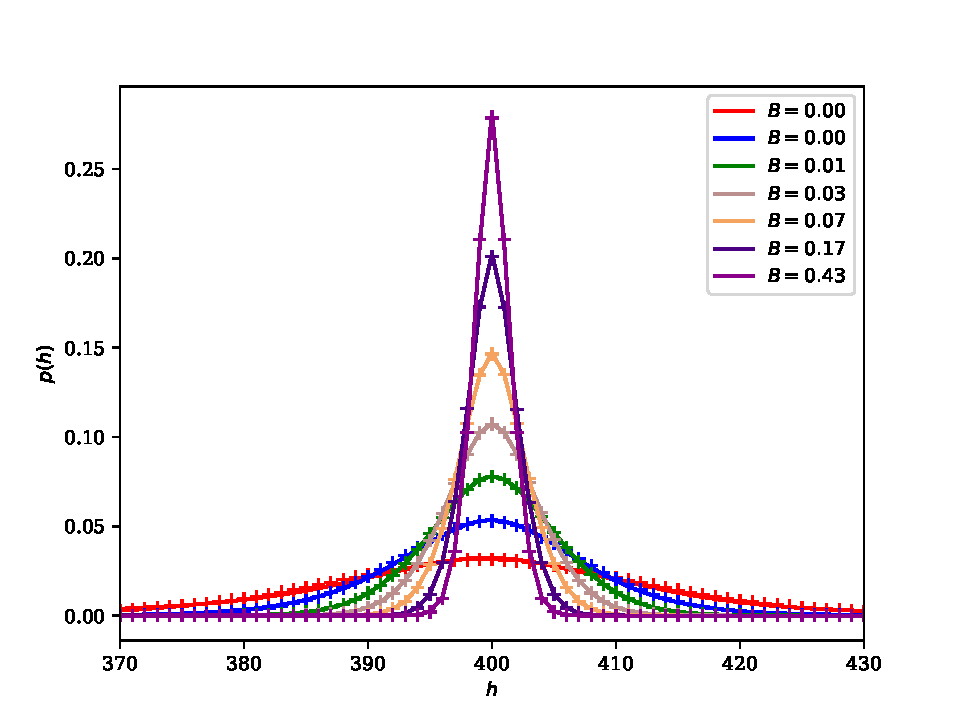
\includegraphics[width=\linewidth]{sosequi-laser/histo.pdf}
	\end{minipage}%
	\begin{minipage}[t]{0.5\linewidth}
		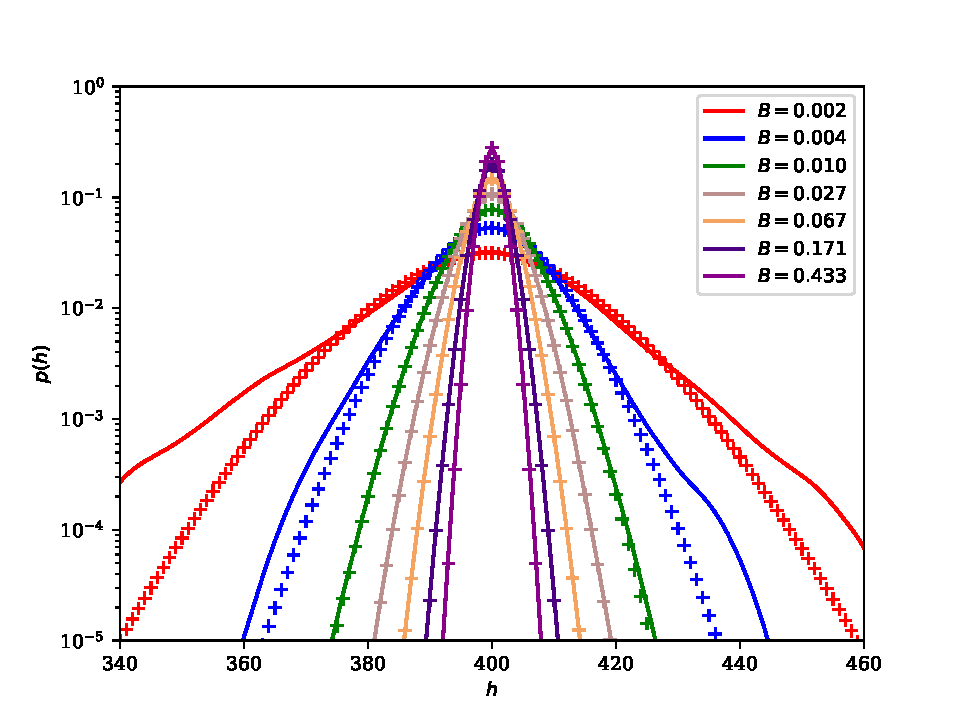
\includegraphics[width=\linewidth]{sosequi-laser/loghisto.pdf}
	\end{minipage}
	\caption{ Distribution de l'interface à $\beta = \beta_C$ autour d'un système centré à $L_Y=400$ en trait plein avec le fit selon la distribution de Airy \ref{airy} en échelle normale (à gauche) et en échelle log (à droite). Les écarts aux grandes fluctuations sont dues à un temps d’échantillonnage trop faible ($10^8$ MC steps) par rapport au temps de corrélation ($T_{cor} \simeq 100$), ce qui ne donne qu'environ $10^6$ états décorrélés. Par comparaison, à haut champ magnétique, le temps de corrélation est $T_{cor} \simeq 2$.}
	\label{histo_airy}
\end{figure}

Lorsque le paramètre d'ordre est conservé, la contrainte des modes de fluctuations dans la fonction de partition change radicalement les propriétés de l'interface. Dans la figure \ref{airy-eq-kae}, on constate la disparité à température et champ magnétique donné entre les ensembles statistiques, dans la limite thermodynamique. {\color{red}  Il semble que l'équivalence des ensembles thermodynamiques ne soit pas vérifiée dans ce système.} Il est possible de trouver une correspondance avec une température et un champ magnétique effectifs différents, mais les propriétés de décroissance à grande distance ne respectent cependant pas la distribution \ref{airy}. 
\begin{figure}
    \centering
	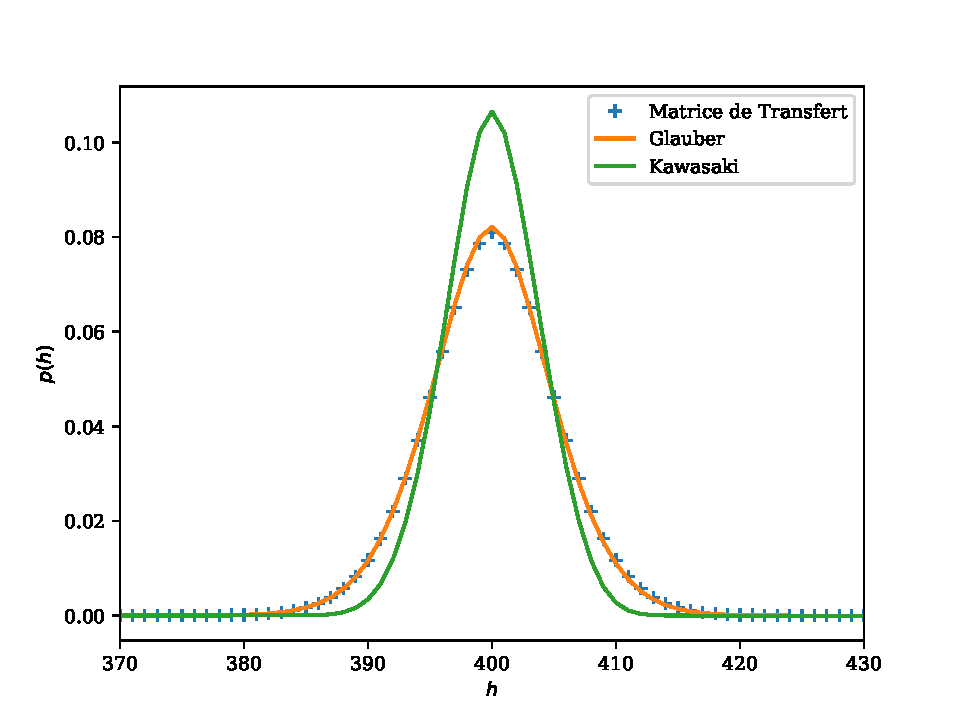
\includegraphics[width=0.5\linewidth]{sosequi-laser/comp-airy-kaw-glau.pdf}
	\caption{Comparaison de la distribution de l'interface entre une dynamique de Glauber et une dynamique de Kawasaki avec conditions aux bords périodiques en $x$ et une géométrie infinie en $y$, avec $L_X=5142$ (la longueur de corrélation parallèle à l'interface est de $\xi_\parallel = 37$ via diagonalisation de la matriice de transfert) pour $T=3$ et $B=0.01$. }
	\label{airy-eq-kae}
\end{figure}

%%%%%%%%%%%%%%%%%%%%%%%%%%
    \subsection{Fonction de corrélation}
%%%%%%%%%%%%%%%%%%%%%%%%%%

On peut également calculer la fonction de corrélation à deux-points. 
D'après l'éq \ref{schro_temp}, l'énergie de chaque état est une longueur caractéristique de chaque mode, $E_0$ étant la plus importante contribution au système. La différence d'énergie entre deux états consécutifs nous donne l'inverse de La longueur de corrélation parallèle à l'interface 
\begin{align}
	\xi_\parallel = \frac{1}{\Delta E} \simeq    2^\frac{1}{3}  \beta^{-\frac{1}{3}} \sigma^{\frac{1}{3}}B^{-\frac{2}{3}}
\end{align}


Dans la limite thermodynamique $L$ grand, la fonction de corrélation  à l'interface est
\begin{align}
	C_f(r) &= \langle f(h(0))f(h(r))\rangle - <f(h(0))><f(h(r))>
\end{align}
Puisque nous sommes dans la limite thermodynamique, la fonction de partition devient $\mZ \simeq e^{-E_0 L}$ et $<f(h(0))> = <f(h(r))> = \int_{-\infty}^\infty dh f(h) \psi_0(h)^2 $.
On obtient alors que
\begin{align}
	C_f(r) &=  \sum_{n\neq 0}\left[\int_{-\infty} ^\infty dh\  f(h)\psi_n(h)\psi_0(h)\right]^2 e^{-(E_n-E_0) r}  \nn
\end{align}
avec $E_n-E_0 = \frac{\alpha_n-\alpha_0}{\xi_\parallel}$. En particulier, si
\begin{align}
	f(h) = {\rm sign}(h-y)
\end{align}
alors $C_f(r)=C(y,r)$ est la fonction de corrélation spin-spin mesurée parallèlement à l'interface à la hauteur $y$. On peut décomposer l'intégrale en deux parties, et grâce à un changement de variable obtenir
\begin{align}
	\int_{-\infty} ^\infty dh\  f(h)\psi_n(h)\psi_0(h)=  2\int_y ^\infty dh\  \psi_n(h)\psi_0(h)
\end{align}
Puisque les $\psi_n$ sont des fonctions d'onde orthogonales répondant à l'équation de Schrödinger, l'intégrale pour $n\neq 0$ est
\begin{align}
	I(n,y)&= \int_y^\infty dh\psi_n(h)\psi_0(h)  \nn
	&= \frac{1}{2}\frac{\psi_0(x)\psi'_n(y) - \psi_n(x)\psi_0'(y)}{\epsilon_n-\epsilon_0}
\end{align} 
Comme précédement, on notant $z= \frac{y}{\xi_\perp}$, on simplifie la fonction de corrélation en
\begin{align}
	C(z ,r) = \sum_{n\neq 0} \frac{\left[ Ai(|z|-\alpha_0)Ai'(|z|-\alpha_n) -Ai(|z|-\alpha_n)Ai'(|z|-\alpha_0) \right]^2}
{ \int_0^\infty dz Ai^2 ( z-\alpha_0 )2 \int_0^\infty dz Ai^2 ( z-\alpha_n ) (\alpha_n-\alpha_0)^2}e^{-[\alpha_n-\alpha_0] \frac{r}{\xi_{||}}}
\end{align}

La constante de normalisation peut être encore simplifiée. L'intégration par partie donne
\begin{align}
	N_n = \int_0^\infty dz Ai^2 (z -\alpha_n) = [z Ai^2 (z -\alpha_n)]_0^\infty - 2\int_0^\infty dz  z Ai(z -\alpha_n)Ai'(z -\alpha_n)
\end{align}
Le terme aux limites est nul, et en utilisant l'équation d'Airy 
\begin{align}
	Ai''(z) -zAi(z)=0 \implies z Ai(z-\alpha_n) = Ai''(z-\alpha_n) + \alpha_n Ai(z-\alpha_n)
\end{align}
on obtient
\begin{align}
	N_n &= -2\int_0^\infty dz [Ai''(z -\alpha_n)+\alpha_n Ai(z -\alpha_n)] Ai'(z -\alpha_n)  \nn
	&= Ai'^2(-\alpha_n) + \alpha_n Ai^2(-\alpha_n).
\end{align}
où l'on rappelle qu'à cause de les modes pairs et impairs, on a posé $Ai(-\alpha_{2n+1})=0$ et $Ai'(-\alpha_{2n})=0$.
Cela nous donne au final
\begin{align}
	C(z,r) = \frac{1}{\alpha_0 Ai^2(-\alpha_0)} \sum_{n} \frac{\left[ Ai(|z|-\alpha_0)Ai'(|z|-\alpha_n) -Ai(|z|-\alpha_n)Ai'(|z|-\alpha_0) \right]^2}
{(Ai'^2(-\alpha_n) + \alpha_n Ai^2(-\alpha_n))  (\alpha_n-\alpha_0)^2}e^{-[\alpha_n-\alpha_0] \frac{r}{\xi_{||}}}
\end{align}

De plus, puisque $C(0,0)=1$, on démontre l'identité suivante entre les zéros de la fonction de Airy (et non de la dérivée)
\begin{align}
\sum_{n=0}^\infty \frac{1}{(\alpha_{2n+1}-\alpha_0)^2\alpha_0} = 1.
\end{align}

À grande distance, seul le terme premier état excité $n=1$ contribue à la fonction de corrélation, ce qui nous donne
\begin{align}
C(z,r) \approx \frac{1}{\alpha_0 Ai^2(-\alpha_0)}  
        \frac{\left[Ai(\frac{|z|}{\xi_{\perp}} -\alpha_{0})Ai'( \frac{|z|}{\xi_{\perp}}-\alpha_{1})-Ai(\frac{|z|}{\xi_{\perp}} -\alpha_{1})Ai'(\frac{|z|}{\xi_{\perp}} -\alpha_{0}) \right]^2}
        { Ai'^2(-\alpha_{1}) (\alpha_1-\alpha_0)^2}\exp(-[\alpha_1-\alpha_0] \frac{r}{\xi_{||}}).
\end{align}

La fonction de corrélation possède donc une décroissance de la forme
\begin{align}
    C(z,r) \approx A(\frac{z}{\xi_\perp})\exp(-[\alpha_1-\alpha_0] \frac{r}{\xi_{||}})
\end{align}
où $A(x)$ est une amplitude dépendante de la hauteur $z$ par rapport à la hauteur moyenne de l'interface, avec une longueur de corrélation  $\xi_{||}$ à grande distance indépendante de la hauteur. Qui plus est, cette longueur de corrélation peut se calculer via les plus grandes valeurs propres de la matrice de transfert $T_{ij} = J (h_i-h_j)^2 + B \frac{|h_i-\frac{L'}{2}|+|h_j-\frac{L'}{2}|}{2}$ grâce à l'équation \ref{longueur-correl-thermo}, ce qui nous donne à très grande distance la relation
\begin{align}
    \xi_{||} = -  \frac{1}{(\alpha_1-\alpha_0) \ln\left(\frac{\lambda_1}{\lambda_0} \right)} = 2^\frac{1}{3}   \beta^{-\frac{1}{3}} \sigma^{\frac{1}{3}}B^{-\frac{2}{3}}
    \label{xi_parallel}
\end{align}

%%%%%%%%%%%%%%%%%%%%%%%%%%
    \subsection{Tension superficielle effective}
%%%%%%%%%%%%%%%%%%%%%%%%%%

\begin{figure}
	\begin{minipage}[t]{0.5\linewidth}
		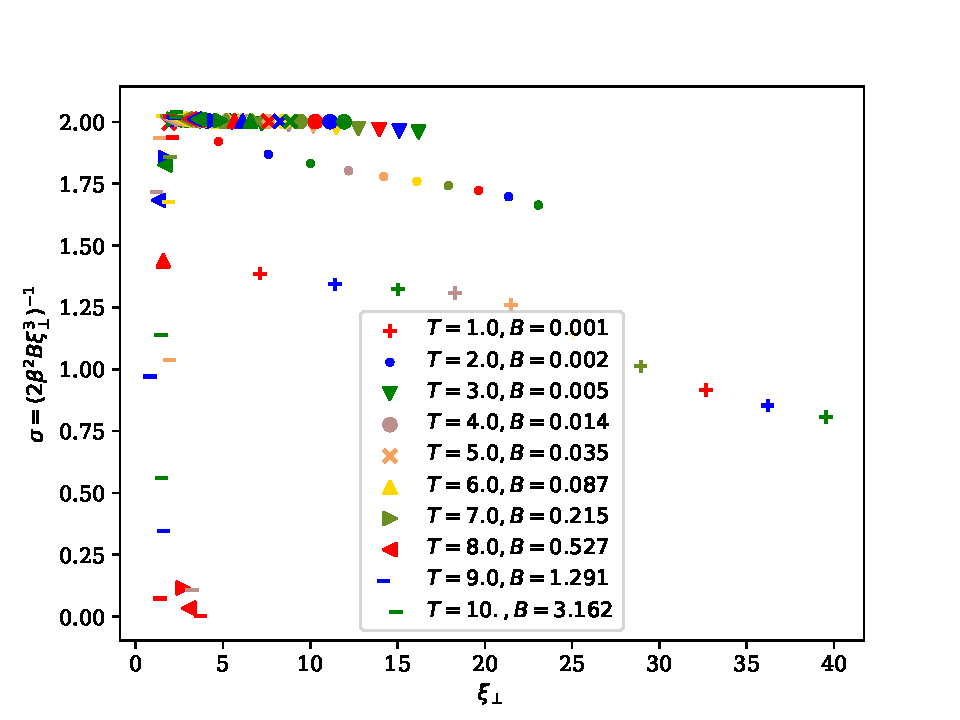
\includegraphics[width=\linewidth]{sosequi-laser/sigma-perp.pdf}
	\end{minipage}%
	\begin{minipage}[t]{0.5\linewidth}
		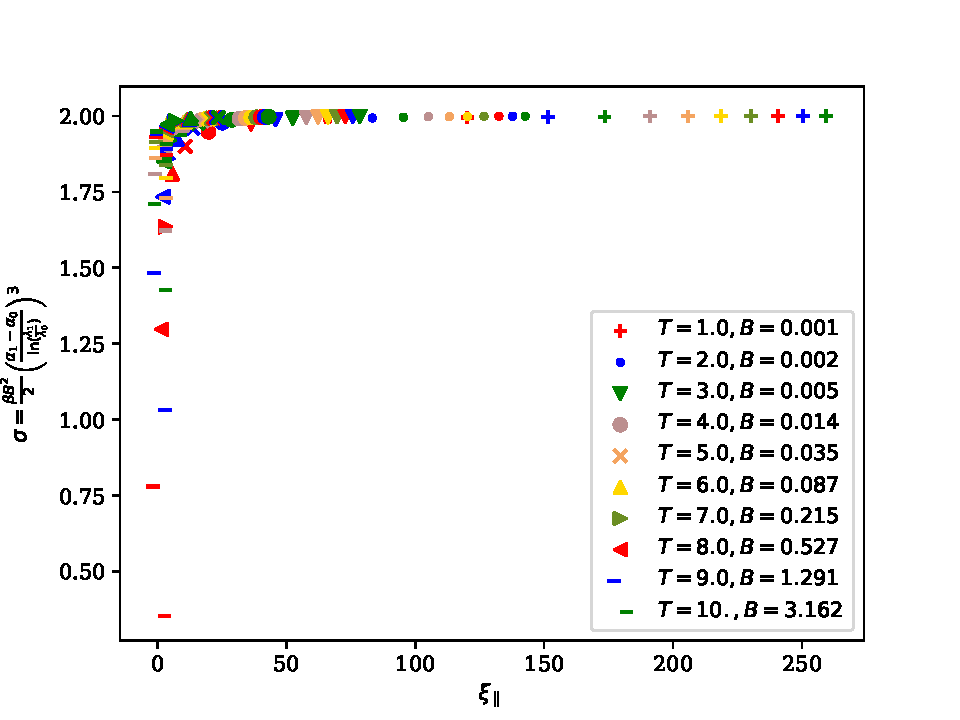
\includegraphics[width=\linewidth]{sosequi-laser/sigma-para.pdf}
	\end{minipage}
	\caption{Vérification des équations \ref{xi_perp} (gauche) et \ref{xi_parallel} (droite) en montrant la tension superficielle $\sigma$ par rapport aux longueurs charactéristiques, calculées grâce à l'Hamiltonien gaussien \ref{hamil-gauss}, pour différentes températures et champs magnétiques, pour une matrice de transfert de talle $L=400$. Chaque couleur correspond à une température, chaque symbole correspond à une intensité du champ magnétique.}
	\label{tension-airy}
\end{figure}

Dans les sections précédentes, nous avons démontré l'existence de deux longueurs de corrélation. La première, $\xi_\perp$, est définie comme la largeur de la distribution d'Airy de l'interface \ref{airy}. La deuxième, $\xi_\parallel$, est définie comme l'inverse de l'écart typique d'énergie entre deux états. En inversant les équatons \ref{xi_perp} et\ref{xi_parallel} on obtient
\begin{align}
    \sigma = \frac{1}{2 \beta^2 B \xi_\perp^3}
\end{align}
et 
\begin{align}
    \sigma = \frac{\beta B^2 (\alpha_1-\alpha_0)^3 \xi_\parallel^3}{2} =  \frac{\beta B^2 (\alpha_1-\alpha_0)^3 }{2 \ln \left(\frac{\lambda_1}{\lambda_0} \right)} 
\end{align}
où $\lambda_0$ est la plus grande valeur propre de la matrice de transfert, et $\lambda_1$ la seconde plus grande valeur propre. Ces deux expressions permettent de croiser les résultats afin de mesurer la tension superficielle effective. Dans la figure \ref{tension-airy}, calcule la valeur de $\sigma$ des deux manières. 
Afin d'obtenir une meilleure précision sur le fit de la distribution, puisque celle-ci est extrêmement piquée autour de la moyenne, il convient de faire le fit sur le logarithme de la distribution afin de donner plus de poids aux valeurs éloignées. On remarque également que pour les températures trop faibles ou des champs trop élevés, la largeur de la dsitribution devient comparable à l'unité, loin de la limite de l'approximation continue $\xi_\perp \gg 1$. Dans le cas où le champ magnétique est trop faible, l'interface est trop faiblement confinée et ne respecte pas non plus la distribution d'Airy. Le plateau que l'on voit sur la figure correspond donc au domaine de validité de l'approximation de la limite continue, où $\sigma = 2 J$. 
Cette valeur de la tension superficielle est corroborée par l'étude de $\xi_\parallel$, qui offre une plus grande robustesse numérique mais demande plus de temps de calcul si l'on désire faire des simulations de Monte Carlo. 

%%%%%%%%%%%%%%%%%%%%%%%%%%%%%%%
    \section{Interface hors-équilibre}
%%%%%%%%%%%%%%%%%%%%%%%%%%%%%%%

La présence d'une force de radiation dans les liquides binaires présentés en introduction induisent un écoulement local des liquides. Cet écoulement est analogue à la décantation de particules dans un solvant, et a pour propriété d'être uniforme. Dans le cas où les deux phases sont séparées et que l'une n'est pas impactée par l'écoulement, on peut considérer un cisaillement que nous définirons plus tard.
Plusieurs études convergent pour dire que la largeur de l'interface d'un tel système diminue avec l'intensité du cisaillement dans les modèles d'Ising \cite{smith_interfaces_2008,smith_interfaces_2008-1}.

Nous avons dans la figure \ref{comp-potentiels-chimiques} que la dynamique de Kawasaki ne peut pas être directement comparée à la dynamique de Glauber pour trouver une tension superficielle directement. Cependant, on peut extraire grâce à l'énergie le comportement global de l'interface vis-à-vis du cisaillement.


Nous nous intéressons au cas d'un écoulement uniforme d'un fluide. L'énergie associée à un écoulement vers la droite du site $i$ au site $j$ est
\begin{align}
    \Delta E_{ec} = f \sgn(i-j)
    \label{ecoulement-uniforme}
\end{align}
Ce genre de cas se retrouve lorsque le vent est en contact avec les vagues ou des nuages, créant une instabilité de Kelvin-Helmoltz augmentant la largeur moyenne de l'interface. Puisque le mouvement induit par l'écoulement peut aller de gauche à droite ou de droite à gauche sans que cela n'affecte l'énergie totale du système, on s'attend à ce que l'énergie soit une fonction paire en fonction de $f$, c'est-à-dire 
\begin{align}
    E(f) = E_{eq} + \frac{f^2}{2} E''(f) + \frac{f^4}{4!} E^{(4)}(f) + ...
\end{align}

\begin{figure}[t]
	\begin{minipage}[t]{0.5\linewidth}
		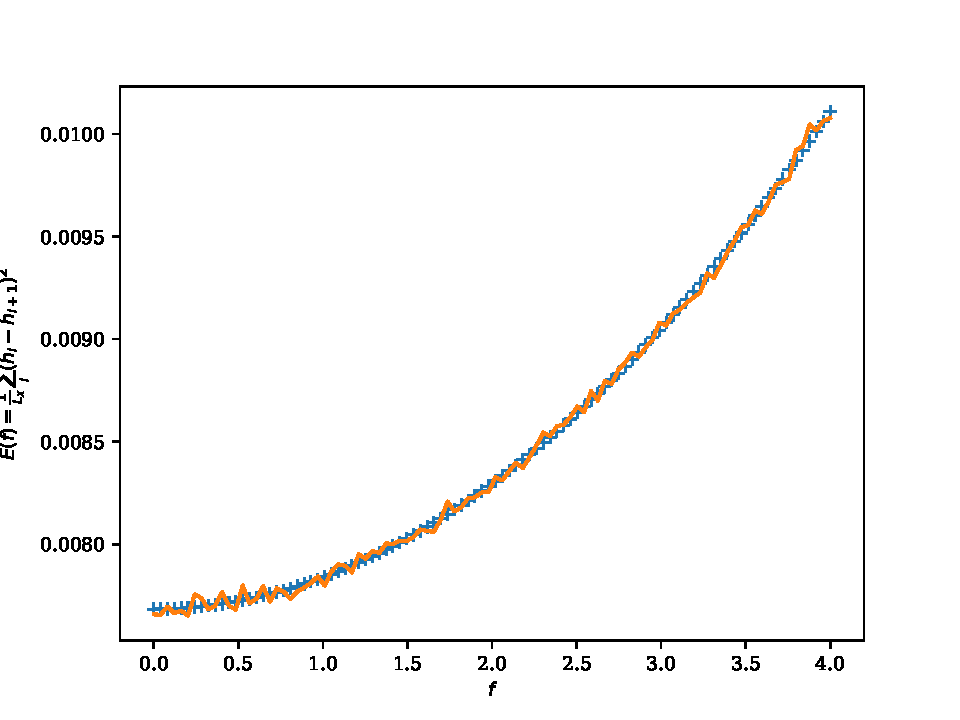
\includegraphics[width=\linewidth]{sosequi-laser/ene-kaw-airy.pdf}
	\end{minipage}%
	\begin{minipage}[t]{0.5\linewidth}
		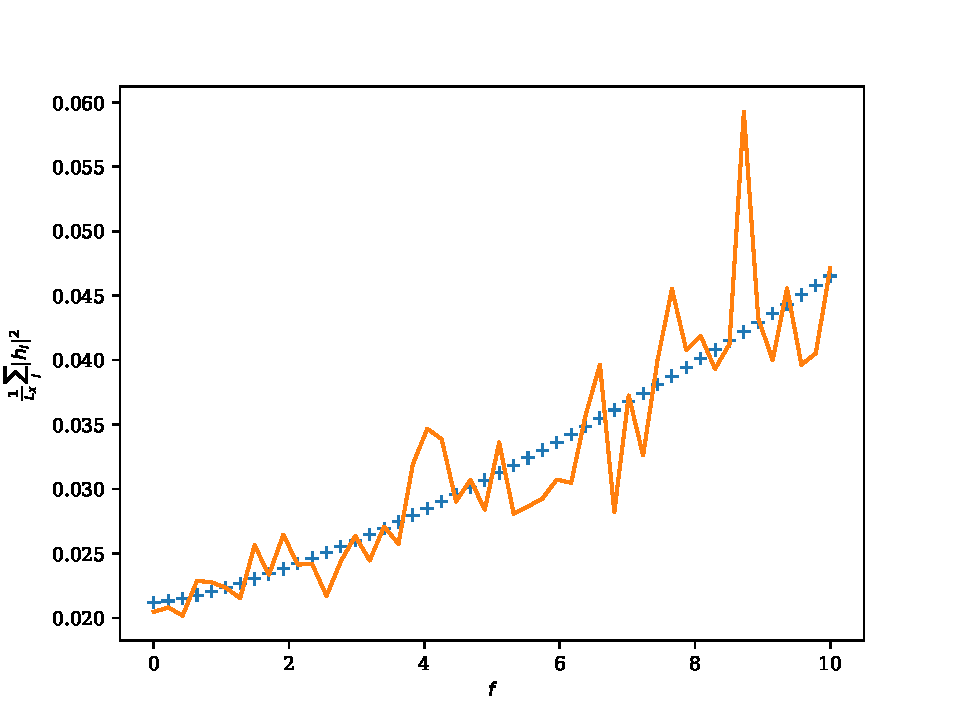
\includegraphics[width=\linewidth]{sosequi-laser/sigma-kaw-airy.pdf}
	\end{minipage}%
	\caption{Énergie par site du modèle gaussien dans une dynamique de Kawasaki pour $T=4$ et $B=0.01$ en fonction de la force \ref{ecoulement-uniforme} -en pointillé un fit avec une puissance carrée (gauche). Largeur de l'interface par site $\frac{1}{L_X}\sum_i |h_i|^2$ en fonction de l'écoulement (droite). {\color{red} Besoin MCIA pour propre,Chip/AiryDrive}}
	\label{ene-kaw-airy}
\end{figure}

Dans la figure \ref{ene-kaw-airy}, on remarque qu'un fit en puissance carrée de dérivée seconde positive explique le comportement général en fonction du cisaillement. On remarque que l'injection d'énergie via l'écoulement vient augmenter l'énergie totale du système, et donc la largeur de l'interface. 
Contrairement au modèle d'Ising, il n'existe ici aucun mécanisme de dissipation de l'énergie. On peut immaginer que dans le modèle d'Ising, la raison pour laquelle le cisaillement diminue la largeur de l'interface \cite{smith_interfaces_2008}, c'est-à-dire diminue la température effective du système \cite{cirillo_monte_2005,winter_finite-size_2010}, est que le cisaillement accélère l'évaporation des cluster. 
Ici, l'énergie est injectée directement au niveau de l'interface et non au bulk, ce qui a tendance, comme avec les vagues, à augmenter la rugosité. 

Si l'on désire instaurer dans nos simlations un écoulement de Couette ou cisaillement, c'est-à-dire une force $\Delta E_{sh}$ qui dépend de la hauteur à laquelle s'effectue le mouvement, il faut insérer dans le modèle une notion de bulk absente des modèles SOS. Nous proposons au prochain chapitre un nouveau modèle capable de prendre en compte différents types de cisaillement.

%%%%%%%%%%%%%%%%%%%%%%%%%%
    \section{Conclusion}
%%%%%%%%%%%%%%%%%%%%%%%%%%

L'interface d'un système définit par un Hamiltonien Solid-On-Solid est une approximation directe du modèle d'Ising, mais décrit mal les systèmes macroscopiques. Afin d'étudier les systèmes continus, nous avons utilisé un Hamiltonien gaussien dont l'intégration est facilement faisable. En utilisant un champ magnétique confinant analogue à l'action d'un laser forçant une phase dans une autre dans les expériences menées au LOMA \cite{girot_conical_2019}, nous avons trouvé que les propriétés de l'interface dans l'ensemble grand-canonique étaient définies par une superposition de modes de Airy. Grâce aux deux longueurs charactéristiques du système étudié, nous avons vérifié l'équivalence entre le modèle continu et le modèle discret puisque $\sigma = 2 J$ dans une grande plage de température et de champ magnétique. Les cas où la correspondance n'est plus valable correspond aux cas où les longueurs charactéristiques sont proches de l'unité, c'est-à-dire que le système est sensible à la discrétisation du système. 
De plus,l es systèmes dans l'ensemble canonique, étudiés grâce à la dynamique de Kawasaki, présentent des propriétés très différentes de celles de l'ensemble grand-canonique. Il peut être intéressant d'explorer la raison pour laquelle l'équivalence des ensembles thermodynamiques est brisée dans ce contexte. L'ajout d'un écoulement uniforme augmente l'énergie et la largeur de l'interface, contrairement aux études sur les modèles d'Ising. Il serait intérssant de vérifier l'hypothèse selon laquelle la diminution de la largeur de l'interface dans les modèles d'Ising est due à l'évaporation accélérée des clusters du bulk.


%\subsection{Discussion about the Gaussian model}
%
%
%
%Pour rappel, à chaque étape on essaie de transférer une particule du site $i$ vers son voisin (gauche ou droit) $j$, ce qui se traduit par $h_i' = h_i-1$ et $h_j' = h_j+1$. 
%Pour $f=0$, en remarquant que les valeurs absolues ont les propriétés suivantes
%\begin{align}
%	|a \pm 1| - |a| = \pm 1 \\
%	|a \pm 2| - |a| = {0,\pm 2}
%\end{align}
%nous voyons facilement l'émergence d'une sélection des énergies possibles entre deux micro-états successifs dans ${-4,-2,0,2,4}$. Ainsi, toutes les transformations diminuant l'énergie totale du système seront toujours acceptées. En augmentant le cisaillement il devient alors possible de refuser des états réduisant l'énergie et d'accepter ceux qui l'augmente. 
%Nous nous attendons alors à trois régimes différents :
%\begin{itemize}
%	\item $f  \less  2 J $ : à faible cisaillement, la symmétrie du système impose les observables à être paire vis-à-vis de $f$, comme le prouve le fit en carré des figures.
%	\item $2 J \less f \less 4 J$ : à cisaillement moyen, certains mouvements augmentant la rugosité de l'interface sont toujours acceptés. 
%	\item $f > 4 J$ : à haut cisaillement, tous les mouvements augmentant l'entropie du système sont acceptés. Une saturation du système se produit lorsque l'énergie de lien entre les sites devient négligeable face au cisaillement.
%\end{itemize}
%
%
%La construction naïve d'un modèle continu du cisaillement avec un seul type de particules ne donnera aucun résultat. En effet, pour que le cisaillement induise des effets hors équilibre, il faut que la dynamique des particules dans tout repère galilén soit le même. Si l'on considère une force de cisaillement uniforme qui induit la même vitesse moyenne sur toutes les particules du système, en nous plaçant dans un repère bougeant à la même vitesse que cette vitesse moyenne, nous retrouvons les mêmes propriétés à l'équilibre.
%Afin de briser la symmétrie de translation, il faut soit induire un cisaillement non-uniforme, soit introduire des particules qui réagissent de manière différente vis-à-vis de cette force. Dans notre exemple sur les colloïdes, la gravité agit bien sur les polymères mais bien moins sur le solvant, ce qui brise en effet l'invariance galiléenne. 
%Plusieurs études récentes portent sur le mouvement de systèmes avec plusieurs particules browniennes, incluant le problème des électrolytes étudié par Onsager \cite{onsager} il y a longtemps.
%
%\begin{figure}[h]
%	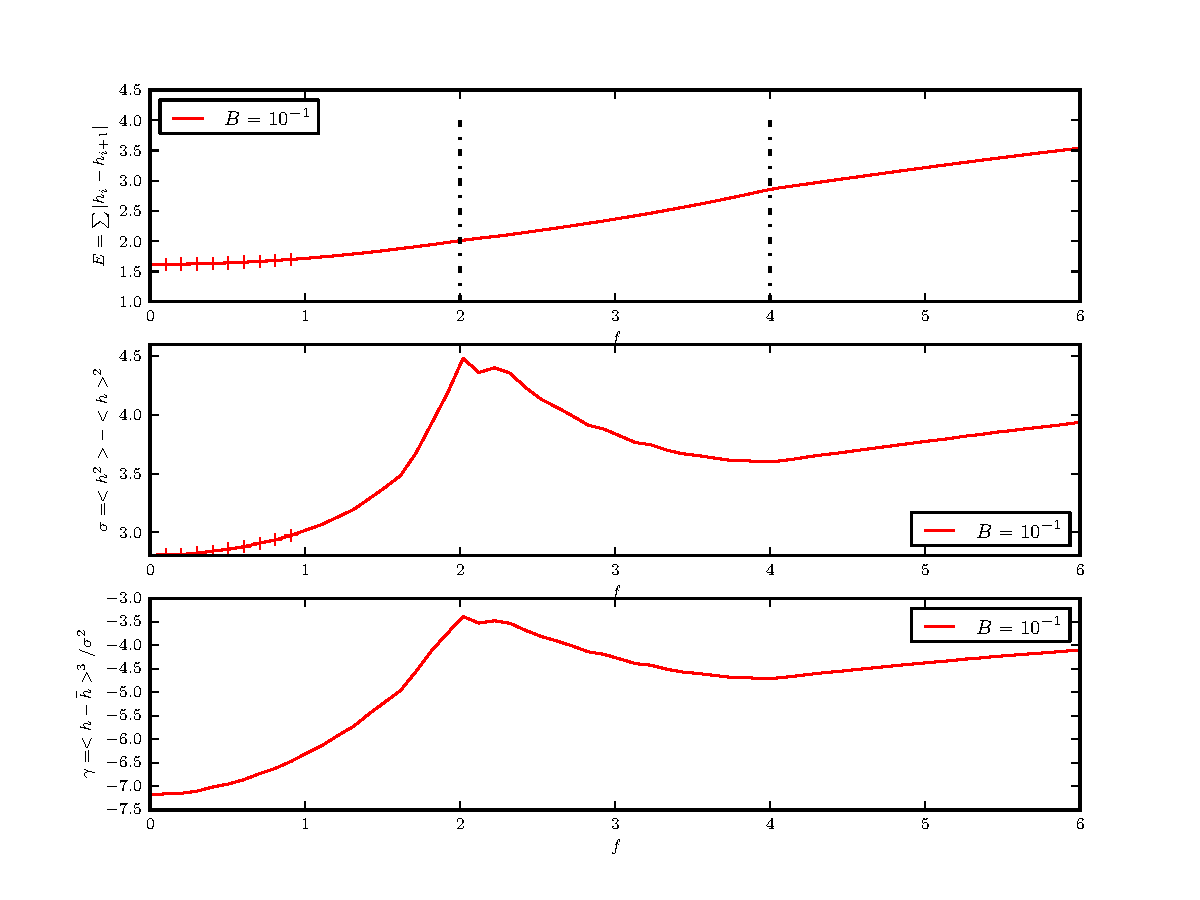
\includegraphics[width=\linewidth]{./sosequi-laser/sosj1.pdf}
%	\caption{Énergie $E= \langle \sum_i |h_i-h_i+1| \rangle$ (en pointillé sa dérivée), variance $\sigma = \langle (H - \langle H \rangle )^2  \rangle$ et asymétrie $\gamma = \langle (H - \langle H \rangle )^3  \rangle / \sigma^2$ pour $B^0.1$. La magnétisation est constante et égale à $\langle H \rangle = 4.51$. Le temps de corrélation du système est presque constant en fonction du cisaillement $f$, allant de  $\tau(f=0) = 5.04$ à $\tau(f=6) = 5.00$ étapes de Monte Carlo. On note une brisure à $f=2J$ et $f=4J$.
%Les croix notent un fit en carré pour petit $f$, montrant la symétrie du système par inversion du signe de $f$. }
%\end{figure}
%
%\begin{figure}
%	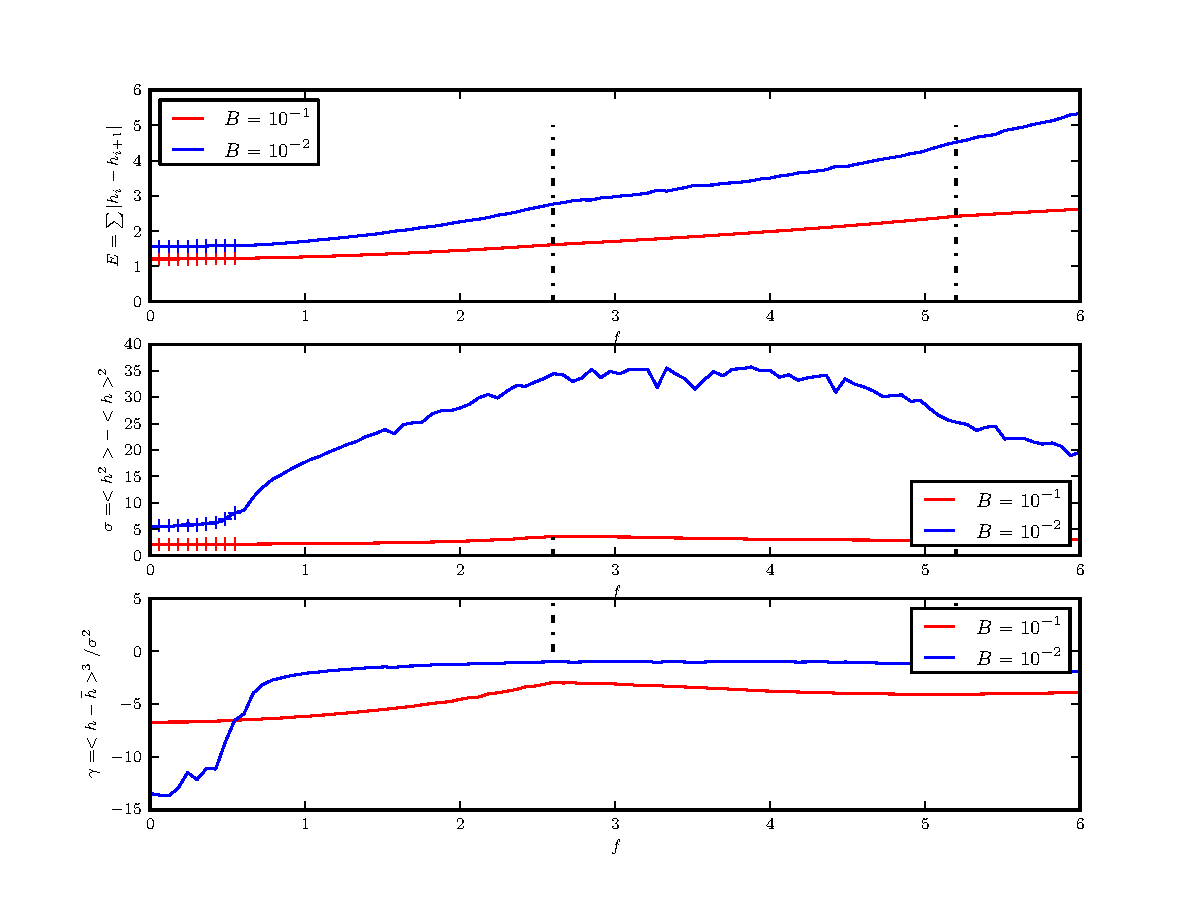
\includegraphics[width=\linewidth]{./sosequi-laser/j13.pdf}
%	\caption{Same as before, with $J=1.3$ We observe a net inflexion in the energy at $2 J$ for  $B=0.01$ which corresponds to $<H>=11$. Nvertheless there is not threshold at $4 J = 5.2$. My guess is that the system is too far away from the boundary in order to interact strongly with it. Interstingly enough, for $B=0.1$, $<H>=3$ and we are too close to the boundaries to see anything.}
%\end{figure}
%
%Instabilité Kelvin-Helmoltz
%	
%The Gaussian model has a stronger interaction, been as
%\begin{align}
%	\Delta E = J \sum (h'_i-h'_{i+1})^2 -(h_i-h_{i+1})^2+ f (i-j)
%\end{align}
%In this model the bond energy between two microstates can take any integer, as 
%\begin{equation*}
%	(h_i-h_j+2)^2 - (h_i-h_j)^2 = 4 (h_i-h_j+1)
%\end{equation*}
%
%The gaussian interaction is very strong, so we could expect a very smooth interface. The mean difference between two sites should be about $h_i-h_{i+1} \simeq 1$. In that case, the energy difference is discretized as ${-8,-4,0,4,8}$. 
%Nonetheless we cannot predict exactly the same behaviour as in the SOS model because this approximation has to be verified everytime, which is false. 1
%
%\begin{figure}
%	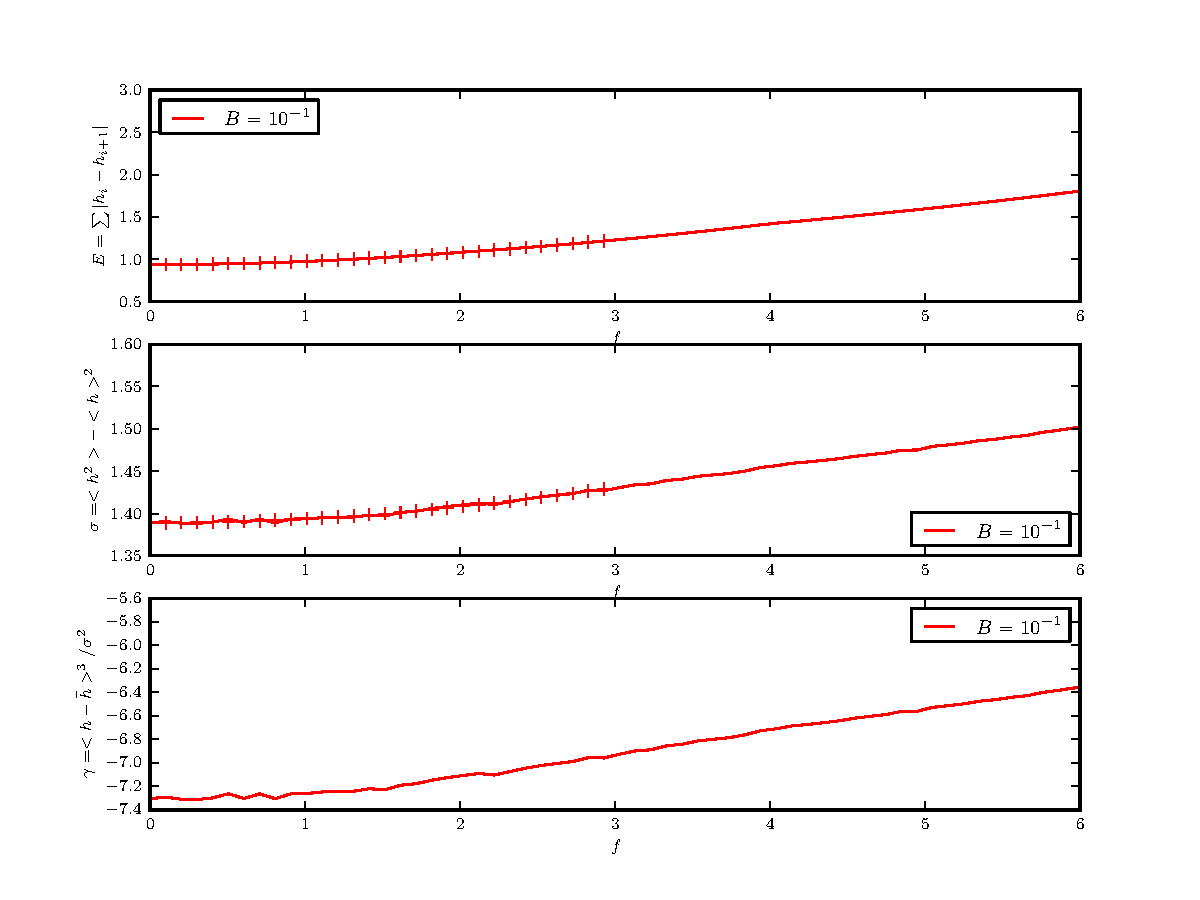
\includegraphics[width=\linewidth]{./sosequi-laser/gauss0.pdf}
%	\caption{Bond energy, thickness (variance) and skewness of the interface for two different magnetic pressures. The magnetisation is constant and is equal to $<H>=2$ for $B=0.1$. As we are very close to the boundary, we see no threshold with the drive force. Simulations take longer with this model because the interaction is stronger}
%\end{figure}
